\section{Background}
\label{sec:background}

\subsection{Blockchain}

At a high level, a blockchain is a sequence of blocks that is immutable in practical applications.
Immutability in blockchains is often provided through Proof of Work.
Proof of Work was introduced in \cite{dwork1992PoW} and first used for blockchain in the Bitcoin whitepaper \cite{nakamoto2009Bitcoin}.
In a Proof of Work blockchain, a block is valid if its cryptographic hash is below a preset threshold.
Each block primarily consists of data that cannot change (financial transactions, medical records, etc).
However, every block contains a field for a fixed-length string of bits that make the output of the hash function below the threshold.
The fixed-length string is called a nonce.
If someone finds a nonce, they have ``mined'' a block.
Since the hash function is cryptographic, it is difficult to reverse.
The best strategy for someone mining a block is to guess and check nonces until a sufficiently low output is found.
Figure \ref{fig:blockchain} displays the typical structure of a blockchain.

\begin{center}
	\vspace{1em}
    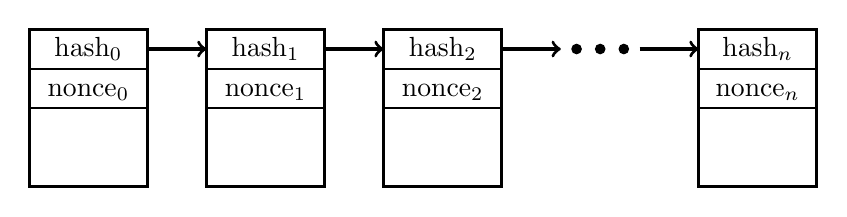
\begin{tikzpicture}
    % blockchain figure

    % boxes (w,l) = (1.5,2)
    \draw [very thick] (0,0) rectangle (1.5,2);
    \node at (0.75,1.75) {hash$_0$};
    \draw [thick] (0,1.5) -- (1.5,1.5);
    \node at (0.75,1.2) {nonce$_0$};
    \draw [thick] (0,1) -- (1.5,1);

    \draw [very thick] (2.25,0) rectangle (3.75,2);
    \node at (3,1.75) {hash$_1$};
    \draw [thick] (2.25,1.5) -- (3.75,1.5);
    \node at (3,1.2) {nonce$_1$};
    \draw [thick] (2.25,1) -- (3.75,1);

    \draw [very thick] (4.5,0) rectangle (6,2);
    \node at (5.25,1.75) {hash$_2$};
    \draw [thick] (4.5,1.5) -- (6,1.5);
    \node at (5.25,1.2) {nonce$_2$};
    \draw [thick] (4.5,1) -- (6,1);

    \draw [very thick] (8.5,0) rectangle (10,2);
    \node at (9.25,1.75) {hash$_n$};
    \draw [thick] (8.5,1.5) -- (10,1.5);
    \node at (9.25,1.2) {nonce$_n$};
    \draw [thick] (8.5,1) -- (10,1);

    % lines (length 0.75)
    \draw [->, very thick] (1.5,1.75) -- (2.25,1.75);
    \draw [->, very thick] (3.75,1.75) -- (4.5,1.75);
    \draw [->, very thick] (6,1.75) -- (6.75,1.75);
    \draw [->, very thick] (7.75,1.75) -- (8.5,1.75);

    % dots
    \draw [fill=black] (6.95,1.75) circle (0.06);
    \draw [fill=black] (7.25,1.75) circle (0.06);
    \draw [fill=black] (7.55,1.75) circle (0.06);

    \end{tikzpicture}
    \captionof{figure}{Prototypical Proof of Work Blockchain \label{fig:blockchain}}
\end{center}


A broader perspective of a blockchain is an implementation of a finite state machine.
In the state machine, blocks are transitions between the states of applications running on top of a blockchain.
Abstractly, the $k^{th}$ block $B_k$ is a transition from state $S_{k-1}$ to state $S_k$ with certain validity requirements.
See Figure \ref{fig:statemachine} for a visual.
A tangible example is a cryptocurrency.
Cryptocurrencies realize state as a record of the amount of currency each public key controls.
Blocks are a set of transactions that transfer currency between public keys.
In state $S_0$, no one controls any currency.
Then block $B_1$ moves the blockchain to $S_1$ where its miner controls some newly created currency.
Then block $B_2$ grants cryptocurrency to its miner and contains currency transfers between users of the currency.
This process repeats until state $S_n$ is reached, which contains the current account-balance pairs of all the current users of a cryptocurrency.

\begin{center}
    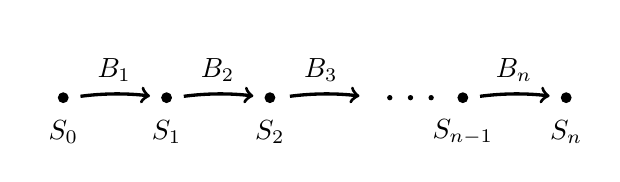
\begin{tikzpicture}[scale=1.75]
        % draw the 0 point
        \draw [thick,color=white] (0,0) -- (0,0);

        % state 0
        \draw [fill=black] (0.25,-0.5) circle (0.035);
        \node at (0.25,-0.75) {$S_0$};

        % block 1
        \draw [very thick, ->] (0.375,-0.49) arc (97.5:83:2);
        \node at (0.62,-0.3) {$B_1$};

        % state 1
        \draw [fill=black] (1,-0.5) circle (0.035);
        \node at (1,-0.75) {$S_1$};

        % block 2
        \draw [very thick, ->] (1.125,-0.49) arc (97.5:83:2);
        \node at (1.37,-0.3) {$B_2$};

        % state 2
        \draw [fill=black] (1.75,-0.5) circle (0.035);
        \node at (1.75,-0.75) {$S_2$};

        % block 3
        \draw [very thick, ->] (1.895,-0.49) arc (97.5:83:2);
        \node at (2.12,-0.3) {$B_3$};

        % ...
        \draw [fill=black] (2.62,-0.5) circle (0.015);
        \draw [fill=black] (2.77,-0.5) circle (0.015);
        \draw [fill=black] (2.92,-0.5) circle (0.015);

        % state n-1
        \draw [fill=black] (3.15,-0.5) circle (0.035);
        \node at (3.15,-0.75) {$S_{n-1}$};

        % block n
        \draw [very thick, ->] (3.275,-0.49) arc (97.5:83:2);
        \node at (3.52,-0.3) {$B_n$};

        % state n
        \draw [fill=black] (3.90,-0.5) circle (0.035);
        \node at (3.90,-0.75) {$S_n$};

    \end{tikzpicture}
    \captionof{figure}{Blocks as transitions between states \label{fig:statemachine}}
\end{center}


\subsection{Technical Problem}

To understand the technical problem, we must understand two properties of blockchains.
First, we observe that miners must have every block in the chain to contribute new blocks.
And, second, blockchains grow in perpetuity.
These properties mean that new miners must download and process an ever increasing amount of data as time passes.
Even now, when Bitcoin is just over a decade old, it can take days or weeks to become a miner.
Such a barrier prevents some nodes from mining, limiting decentralization.
Less decentralization reduces the effectiveness of a blockchain.

When viewing a blockchain as a finite state machine, we can change the requirements of what a miner needs to know.
All a miner must know is a state $S_k$ and every block following that state.
Then a bootstrapping miner could compute the current state.
If $S_k$ is close to the end of the chain, then the miner requires significantly less bootstrapping time by only requesting blocks following $S_k$.

How does a bootstrapping miner obtain the state $S_k$?
They can't just ask a blockchain node, because they could receive a faulty state.
This is the problem we would like to solve: Can we provide a mechanism so that a bootstrapping node can trust a recent state?

\subsection{Related Work}

% lightweight nodes in the bitcoin whitepaper

% summary block in the main chain

% miniblockchain

% separate summary chain

% coinprune 

Our solution gains inspiration from a paper written by Matzutt et al. that provides a way to verify Bitcoin states.
They suggest that recent miners be allowed to vote for a state and then bootstrapping nodes trust the majority of votes.
Each vote is recorded in a block and each block has the capacity to store a single vote \cite{matzutt2020HowTSPrune}.
Storing votes in blocks gives them immutability, so a bootstrapping node knows that they are counting every vote.

There are two problems with this idea.
First, a vote can only be generated as quickly as new blocks.
In Bitcoin, this averages to about 10 minutes per block, meaning a bootstrapping node might have to wait a week for there to be sufficiently many votes to trust a state.
Second, this solution relies on implementation details in the Bitcoin protocol and may not apply to blockchains in general.
